\chapter{Budowa urządzenia}

\section{Konstrukcja}

Część mechaniczna urządzenia została zamodelowana w programie Solidworks, dzięki czemu ustalono jakie elementy konstrukcyjne są potrzebne oraz czy nie występują kolizje z poruszającym się wózkiem. Koncepcyjny model 3D zaprezentowano na rysunku \ref{fig:konstrukcja}. 

\begin{figure}
    \centering
    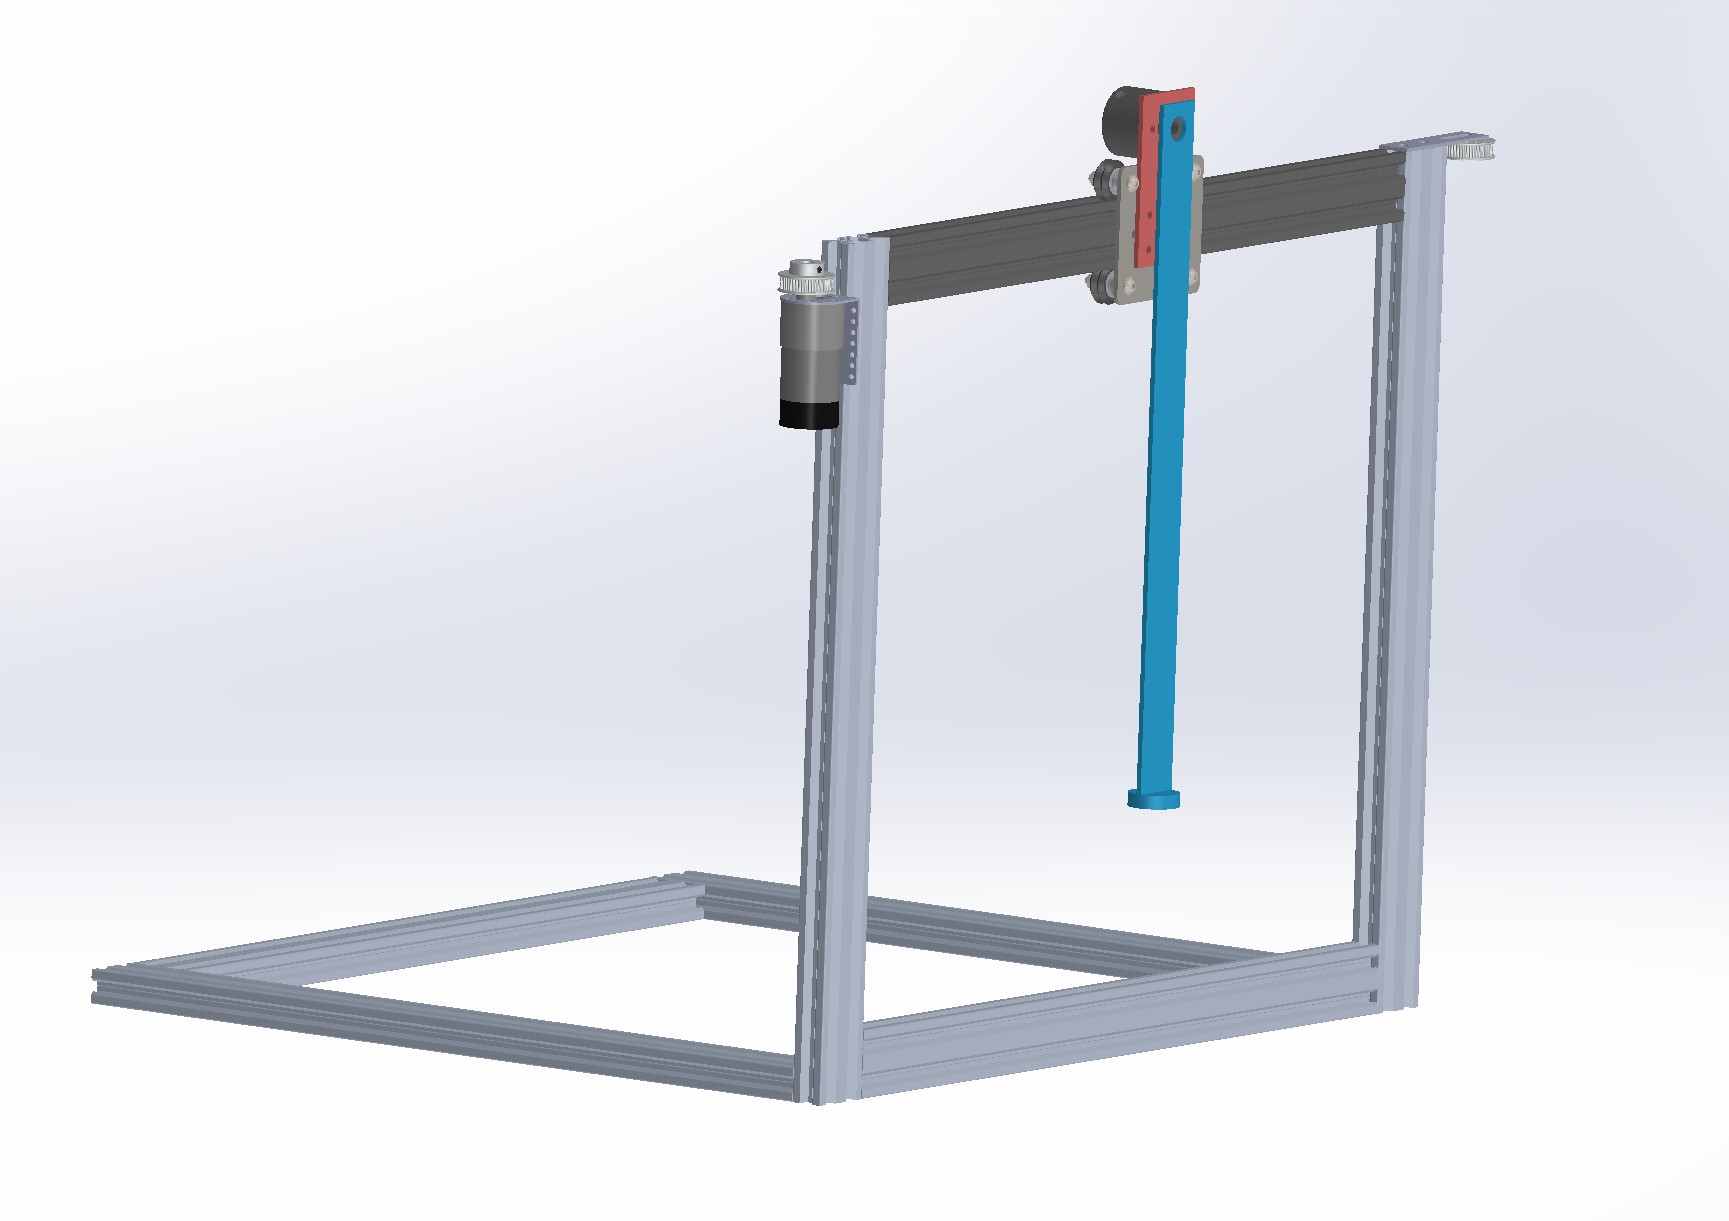
\includegraphics[scale=0.5]{praca_dyplomowa/figures/pendulum6.jpg}
    \caption{Poglądowy model 3D konstrukcji}
    \label{fig:konstrukcja}
\end{figure}

\subsection{Rama}
Do budowy konstrukcji urządzenia zostały wykorzystane aluminiowe profile typu V-Slot 2040, jak na rysunku \ref{fig:profil}. Przekrój profilu ma wymiary 20 x 40 mm, a jego boki mają charakterystyczne rowki w kształcie litery V. Rama została zbudowana z 3 profili o długości 500mm oraz 4 profili długości 250mm. Wszystkie elementy zostały ze sobą połączone dedykowanymi elementami wydrukowanymi na drukarce 3D oraz śrubami M4. Część elementów łączeniowych została znaleziona na stronie \textit{thingiverse.com}, na której udostępniane są modele 3D przygotowane z myślą o ich wydrukowaniu. Konstrukcja złożona w ten sposób charakteryzuje się dużą sztywnością, a przy tym niską masą.

\begin{figure}
    \centering
    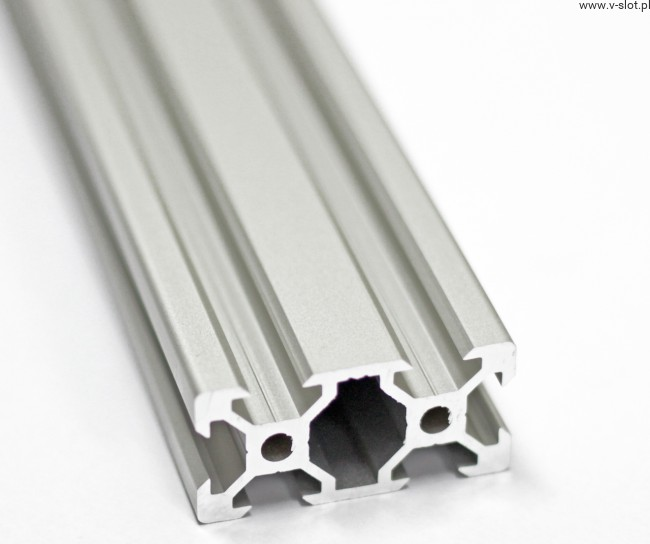
\includegraphics[scale=0.7]{praca_dyplomowa/figures/profil.jpg}
    \caption{Aluminiowy profil 2040}
    \texttt{Źródło: v-slot.pl}
    \label{fig:profil}
\end{figure}

\subsection{Układ jezdny}
Poruszający się wózek, popularnie nazywany karetką, został zbudowany na stalowej blasze, do którego przymocowano 4 łożyskowane rolki widoczne na rysunku \ref{fig:Rolka}, które są dedykowane do poruszania się po profilach V-Slot. Dodatkowo dolne rolki zostały zamontowane na tulejach mimośrodowych, dzięki czemu można regulować siłę docisku rolek do profilu. Do karetki przymocowany pas zębaty GT2 o szerokości 6mm, który z jednej strony porusza się po kole pasowym będącym napinaczem, a z drugiej po kole zębatym, które jest zamontowane na wale silnika. 

\begin{figure}
    \centering
    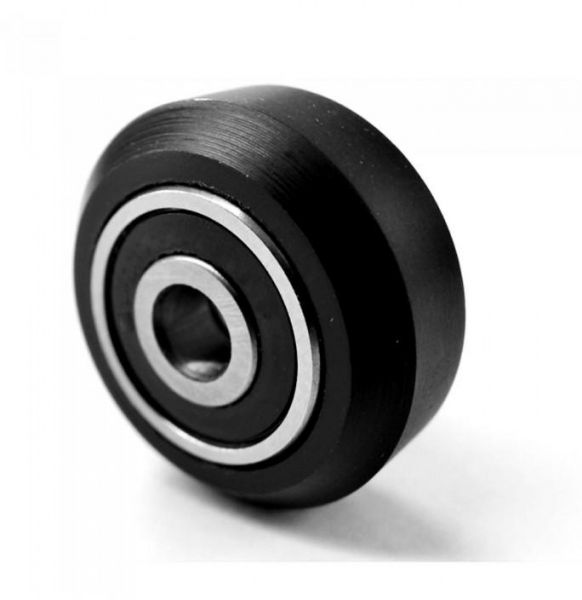
\includegraphics[scale=0.3]{praca_dyplomowa/figures/wheel.jpg}
    \caption{Rolka jezdna}
    \texttt{Źródło: black-frog.pl}
    \label{fig:Rolka}
\end{figure}

\section{Podzespoły}

\subsection{Mikrokontroler}
\label{sec:STM32}
W urządzeniu został wykorzystany mikrokontroler firmy STMicroelectronics STM32F407 Discovery ukazany na rysunku \ref{fig:STM32}. Moduł wyposażony jest w 32-bitowy rdzeń ARM Cortex M4F. Maksymalne taktowanie mikroprocesora to 168 MHz, oferuje 1 MB pamięci flash oraz 192 kB pamięci RAM. Dodatkowo moduł jest wyposażony w dedykowany programator ST-LINK/V2, który pozwala również na debuggowanie. Mikrokontroler oferuje wiele programowalnych wejść i wyjść, a w tym między innymi w trybie wejścia sygnału enkodera czy wyjścia sygnału PWM. Moduł można zasilać zarówna z 5V jak i 3,3V. Płytka wraz ze sterownikiem silnika zostały przymocowane do konstrukcji przy pomocy samodzielnie zaprojektowanego uchwytu. 

\begin{figure}
    \centering
    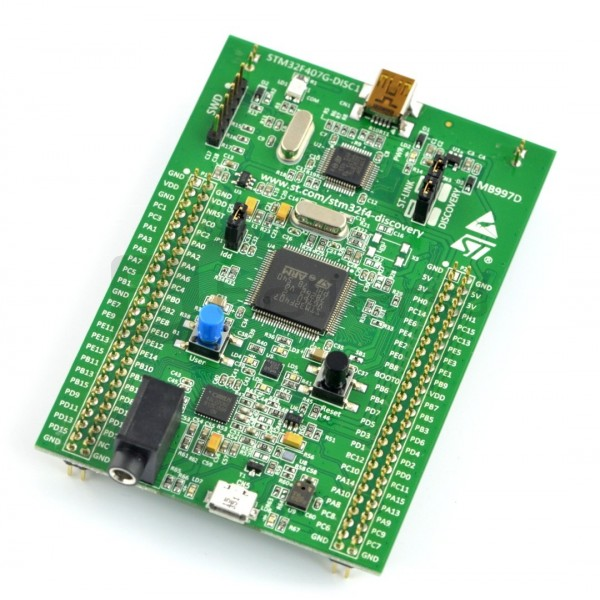
\includegraphics[scale=0.8]{praca_dyplomowa/figures/STM32F407.jpg}
    \caption{Mikrokontroler STM32F407 Discovery}
    \texttt{Źródło: botland.com.pl}
    \label{fig:STM32}
\end{figure}

\subsection{Enkoder}
Jako czujnik kąta odchylenia wahadła został wykorzystany enkoder DFRobot 400P/R, przedstawiony na rysunku \ref{fig:Enkoder}. Czujnik ma rozdzielczość 400 impulsów na każdy z 2 kanałów. Na wyjściach generowane są sygnały kwadraturowe, które są przesunięte w fazie względem siebie o 90\degree. W zależności od tego, na którym kanale najpierw pojawia się sygnał można rozróżnić kierunek obrotów. Przy zliczaniu zliczaniu wszystkich zboczy sygnałów maksymalna rozdzielczość wynosi 1600 impulsów na obrót z czego wynika, ze jeden impuls to odchylenie o 0,225\degree. Enkoder może być zasilany napięciem od 4,8V do 24V. Sygnały wyjściowe czujnika są generowane przez tranzystory NPN w układzie otwartego kolektora, przez co linie sygnałowe wymagają podciągnięcia przez rezystory do dodatniej linii zasilania (pull-up).

\begin{figure}
    \centering
    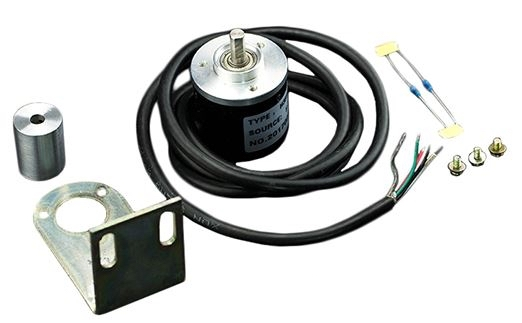
\includegraphics[scale=0.7]{praca_dyplomowa/figures/encoder.jpg}
    \caption{Enkoder DFRobot 400P/R}
    \texttt{Źródło: jsumo.com}
    \label{fig:Enkoder}
\end{figure}

\subsection{Silnik}
Do poruszania karetką został wykorzystany silnik prądu stałego Pololu 37Dx65L, ukazany na rysunku \ref{fig:Silnik}. Napięcie zasilania silnika to 12V, minimalny pobór prądu to 0,2A, a maksymalny przy zatrzymaniu wału 5,5A. Silnik wyposażony jest w przekładnię o przełożeniu 6,25:1, dzięki której osiąga 1600 RPM przy nominalnym napięciu, a moment obrotowy wynosi 3kg/cm, czyli 0,294Nm. Dodatkowo silnik posiada własny enkoder o rozdzielczości 16 impulsów na obrót na każdym kanale co maksymalnie daje 64 impulsy na pełny obrót. Enkoder silnik może być zasilany napięciem od 3,5V do 20V. 

\begin{figure}
    \centering
    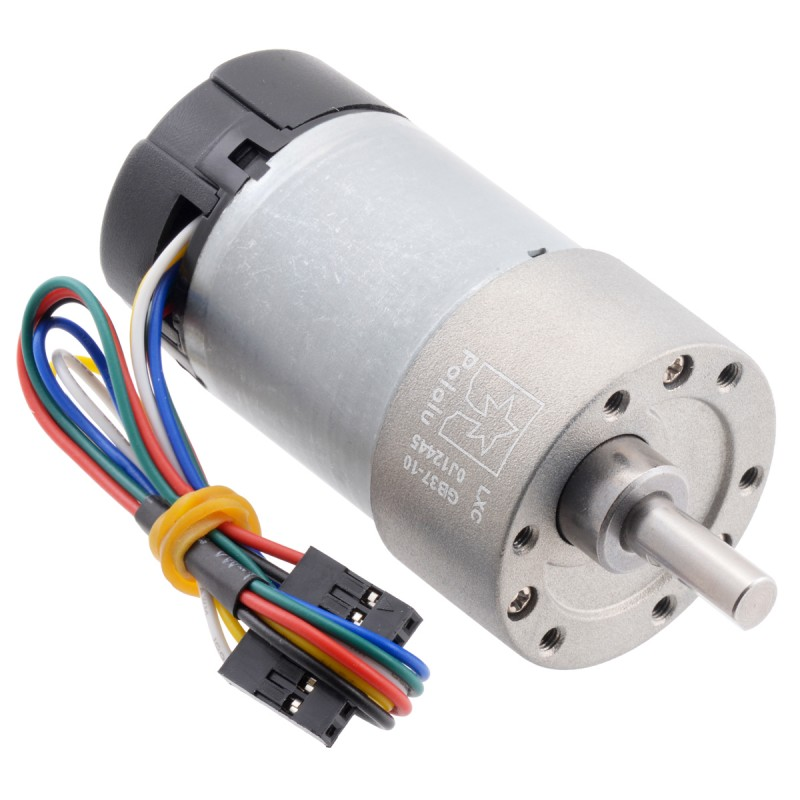
\includegraphics[scale=0.3]{praca_dyplomowa/figures/Pololu 37D.jpg}
    \caption{Silnik DC Pololu 37D}
    \texttt{Źródło: kamami.pl}
    \label{fig:Silnik}
\end{figure}

\subsection{Sterownik silnika}
Do sterowania silnikiem DC został wykorzystane moduł wyposażony w sterownik L298N, widoczny na rysunku \ref{fig:L298N}. Układ ten umożliwia sterowanie 2 silnikami dzięki dwóm osobnym kanałom. Napięcie zasilania silników może być dowolne z przedziału 4,8V do 46V, natomiast część logiczna wymaga zasilania napięciem 5V. Maksymalny prąd wyjściowy to 2A na każdy kanał, a dodatkowo kanały można połączyć ze sobą równolegle przez dwukrotnie zwiększy się wydajność prądowa. Moduł, dzięki zastosowaniu mostka H, pozwala sterować silnikiem w różnych kierunkach, a także stosować szybkie lub wolne hamowanie. Prędkość obrotów silnika można regulować sygnałem PWM.

\begin{figure}
    \centering
    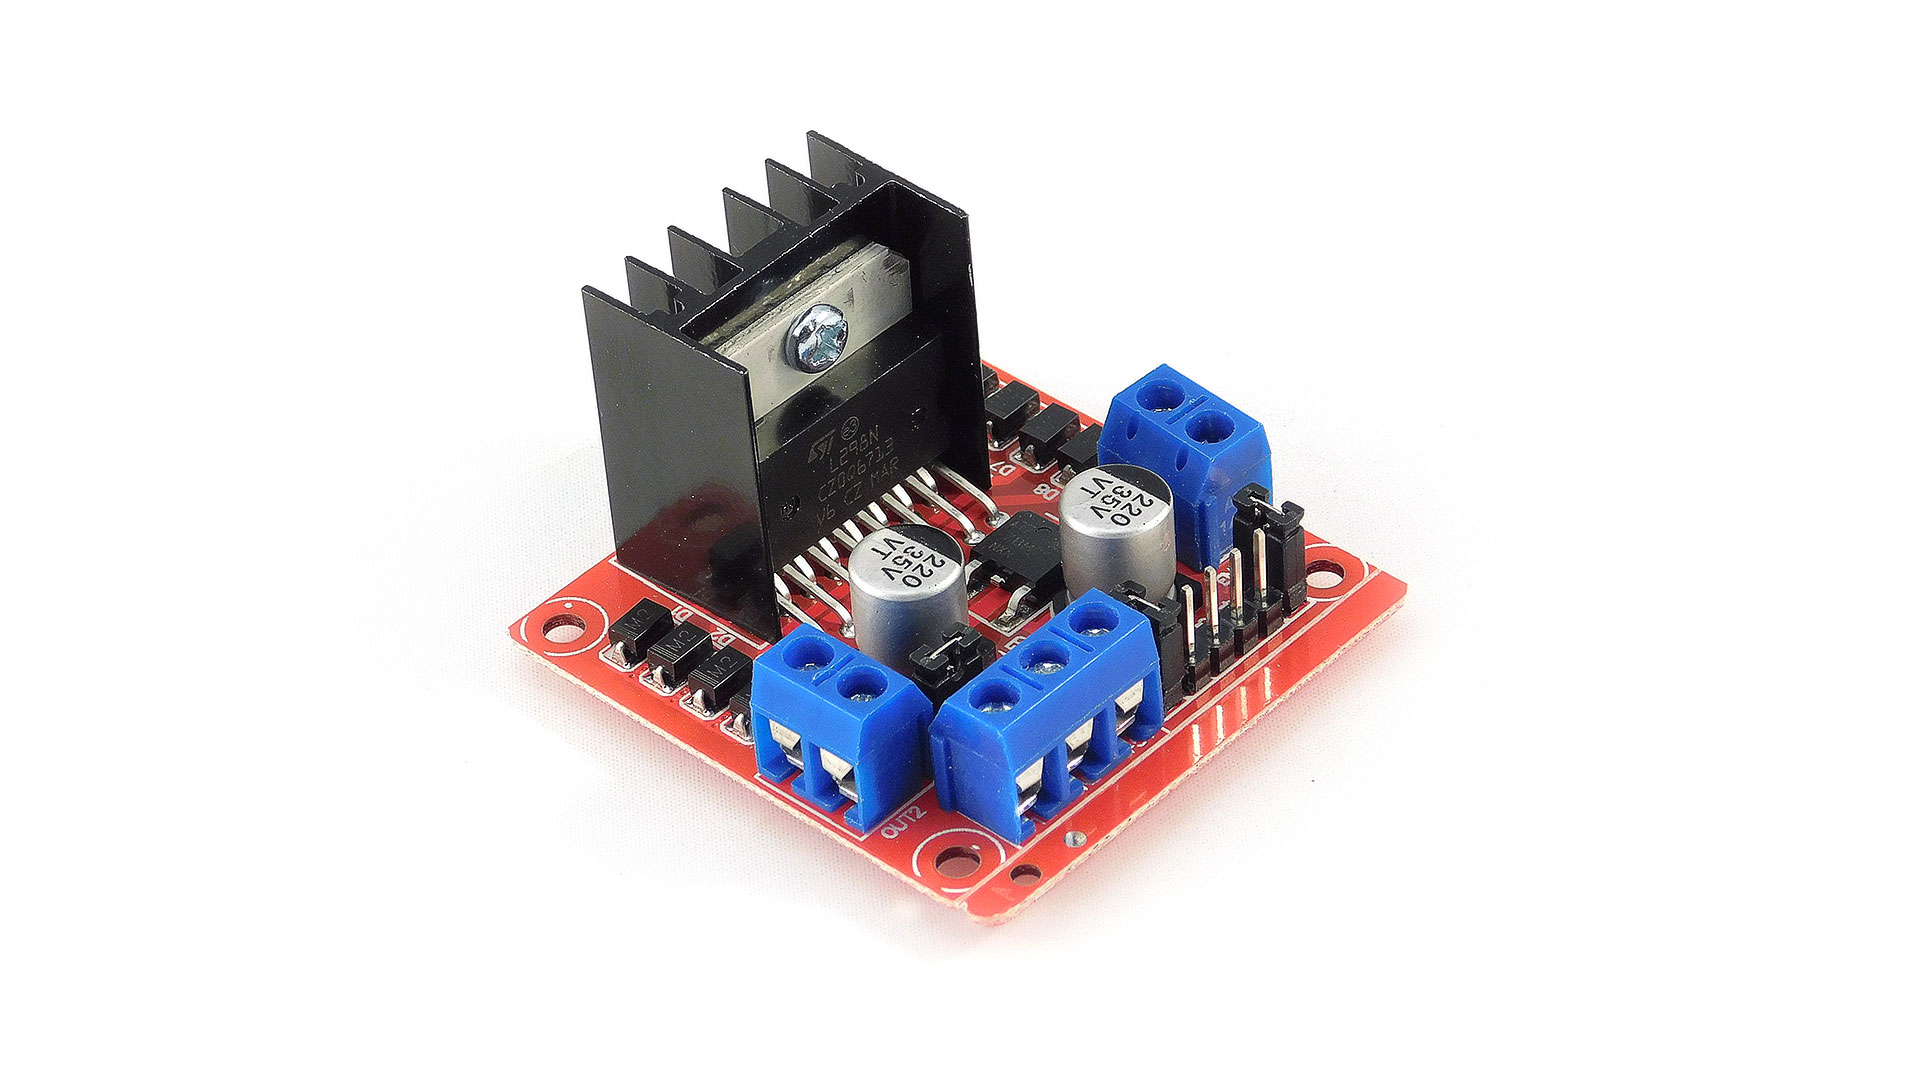
\includegraphics[scale=0.2]{praca_dyplomowa/figures/L298N.JPG}
    \caption{Sterownik silników DC L298N}
    \texttt{Źródło: botland.com.pl}
    \label{fig:L298N}
\end{figure}

\subsection{Zasilacz}
Do zasilania wszystkich podzespołów został użyty zasilacz komputerowy ATX o maksymalnej mocy 400W jak na rysunku \ref{fig:zasilacz}. Zaletą tego rozwiązania jest zapewnienie potrzebnych różnych napięć zasilania, bez potrzeby stosowania dodatkowych przetwornic. Zasilacz został umocowany do ramy przy pomocy samodzielnie zaprojektowanego i wydrukowanemu uchwytu.

\begin{figure}
    \centering
    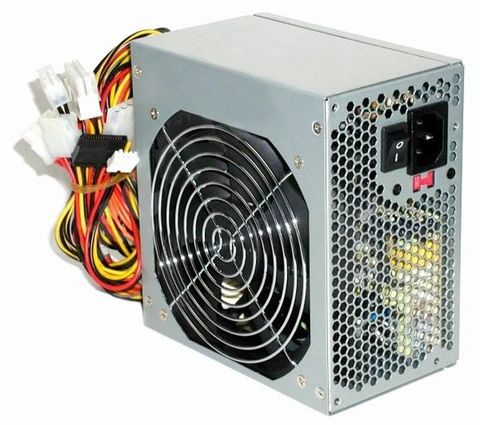
\includegraphics[scale=0.8]{praca_dyplomowa/figures/zasilacz.jpg}
    \caption{Zasilacz ATX 400W}
    \texttt{Źródło: internet-chorzow.pl}
    \label{fig:zasilacz}
\end{figure}

\section{Dodatki}
Do konstrukcji został dołączony mini komputer Raspberry Pi 4. Komunikuje się on z mikrokontrolerem STM32 poprzez magistrale UART. Wybór protokółu komunikacji wynika z łatwości implementacji w obu urządzeniach. Ponadto, do komunikowania się mikrokontrolera i komputera nie jest wymagana duża szybkość przesyłu. Protokół UART został skonfigurowany w następujący sposób na obu urządzeniach:
\begin{itemize}
    \item szybkość transmisji 115200 Bps
    \item 8 bitów
    \item 0 bitów parzystości
\end{itemize}

Komunikacja pomiędzy urządzeniami wykorzystana jest do edycji współczynników wpływających na regulację wahadła. Na ekranie dostępne są suwaki, które odpowiedzialne są za współczynniki algorytmu sterowania. Oprócz tego widoczne sa 3 przyciski:
\begin{itemize}
    \item \textit{SEND} -- wysyła nowe ustawienia,
    \item \textit{GET} -- pobiera aktualne ustawienia,
    \item \textit{SET 0} -- resetuje pomiar wychylenia wahadła.
\end{itemize}
Opcja \textit{Send} wysyła nowe współczynniki całego algorytmu w postaci ramki danych: \[H\,pp\,pi\,pd\,mp\,md\,wsp\]
gdzie:
\begin{itemize}
    \item \textit{H} -- nagłówek wiadomości,
    \item \textit{pp} -- nastawa członu proporcjonalnego regulatora wahadła, 
    \item \textit{pi} -- nastawa członu całkującego regulatora wahadła,
    \item \textit{pd} -- nastawa członu różniczkującego regulatora wahadła,
    \item \textit{mp} -- nastawa członu proporcjonalnego regulatora położenia,
    \item \textit{md} -- nastawa członu różniczkującego regulatora położenia,
    \item \textit{wsp} -- stosunek regulatora położenia do regulatora wahadła.
    \label{it:ramka}
\end{itemize}
Nagłówek wiadomości to informacja dla mikrokontrolera, który przycisk został naciśnięty:
\begin{itemize}
    \item \textit{P -- Send} -- zmienia współczynniki algorytmu na te przesłane w wiadomości,
    \item \textit{G -- Get} --  wysyła aktualne ustawienia,
    \item \textit{S -- Set 0} -- resetuje pomiar wychylenia wahadła.
\end{itemize}
W odpowiedzi na każdą nadesłaną wiadomość mikrokontroler odsyła do Raspberry Pi ramkę danych w postaci pliku JSON ("klucz":wartość):
\[\{"pp":44.00,"pi":10.00,"pd":1.20,"mp":16.50,"md":1.00,"wsp":0.80\}\] 
gdzie:
\begin{itemize}
    \item \textit{pp} -- nastawa członu proporcjonalnego regulatora wahadła, 
    \item \textit{pi} -- nastawa członu całkującego regulatora wahadła,
    \item \textit{pd} -- nastawa członu różniczkującego regulatora wahadła,
    \item \textit{mp} -- nastawa członu proporcjonalnego regulatora położenia,
    \item \textit{md} -- nastawa członu różniczkującego regulatora położenia,
    \item \textit{wsp} -- stosunek regulatora położenia do regulatora wahadła.
    \label{it:ramka}
\end{itemize}

Mikrokontroler po otrzymaniu danych i sprawdzeniu ich poprawności wczytuje je jako aktualne ustawienia. 

Aplikacja, która wyświetla i pozwala edytować ustawienia została stworzona w środowisku \textit{Node-Red}, która pozwala w sposób graficzny na zbudowanie funkcjonalnego programu. Środowisko to korzysta z języka \textit{JavaScript}, a budowanie programu polega na łączenie ze sobą odpowiednich bloczków. Każdy blok można odpowiednio skonfigurować, a możliwości całego środowiska rozszerza bogata biblioteka wtyczek. Istnieje również możliwość stworzenia własnego bloku programu, w którym mieści się kod w języku \textit{JavaScript}. Programowanie w środowisku \textit{Node-Red} standardowo dostępne jest na porcie 1880 komputera, na którym się znajduje i korzysta się z niego przez przeglądarkę internetową. Aplikacja zademonstrowana jest na rysnku \ref{fig:nodered}.

\begin{figure}
    \centering
    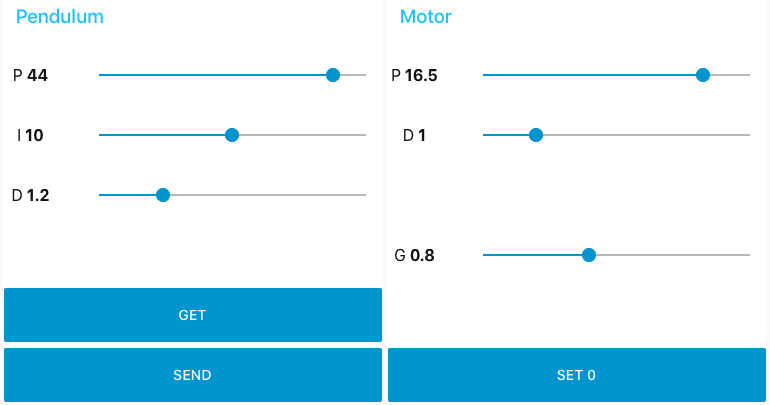
\includegraphics[width=\textwidth]{praca_dyplomowa/figures/nodered.png}
    \caption{Wygląd aplikacji umożliwiającej zmianę nastaw regulatorów}
    \label{fig:nodered}
\end{figure}

\begin{figure}
    \centering
    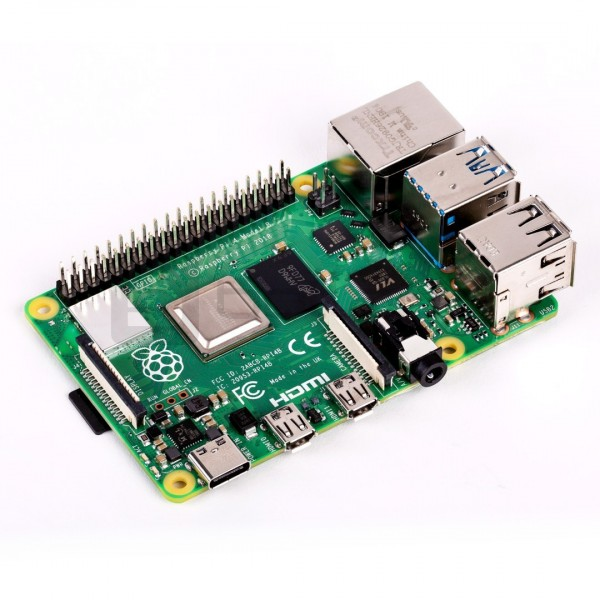
\includegraphics[scale=0.6]{praca_dyplomowa/figures/rpi4.jpg}
    \caption{Raspberry Pi 4 model B}
    \texttt{Źródło: botland.pl}
    \label{fig:rpi4}
\end{figure}

\begin{figure}
    \centering
    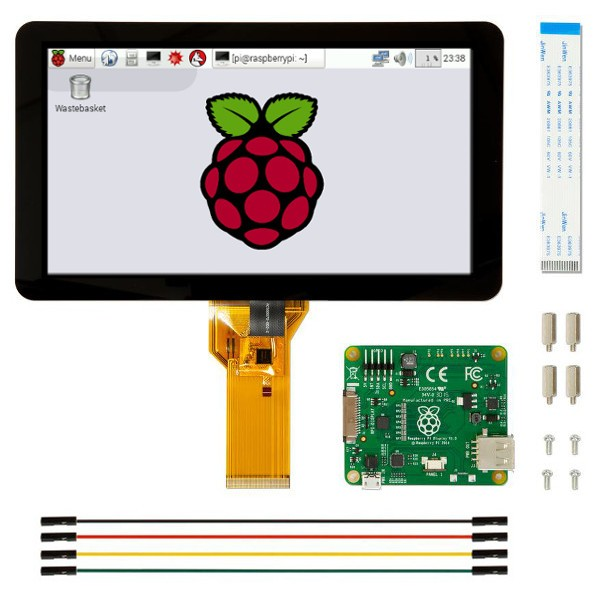
\includegraphics[scale=0.5]{praca_dyplomowa/figures/rpidisplay1.jpg}
    \caption{Dotykowy wyświetlacz Raspberry Pi}
    \texttt{Źródło: botland.pl}
    \label{fig:rpidisp1}
\end{figure}

\begin{figure}
    \centering
    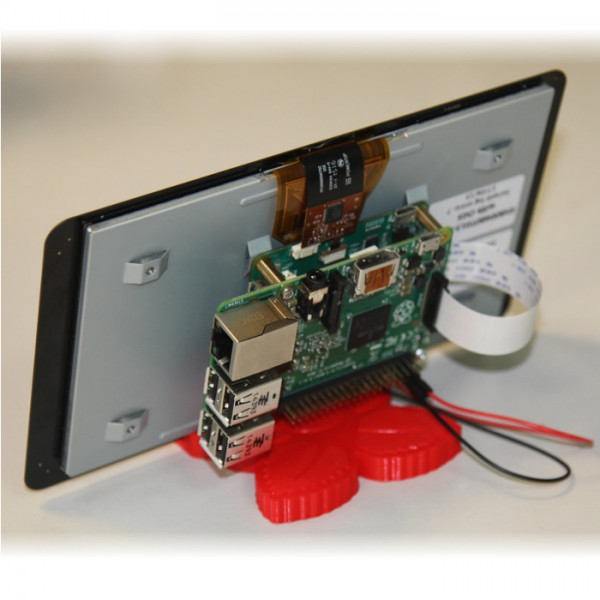
\includegraphics[scale=0.5]{praca_dyplomowa/figures/rpidisplay2.jpg}
    \caption{Dotykowy wyświetlacz Raspberry Pi -- sposób montażu}
    \texttt{Źródło: botland.pl}
    \label{fig:rpidisp2}
\end{figure}